\section[CPU]{Design of a 16 bit Central Processing Unit (CPU)} 
A Central Processing Unit (CPU) is the electronic circuit withing a computer that executes instructions that make up a computer.The CPU, by all means, is one of the most important component of a computer system. Since computers vary from one another by size and complexity, so does there CPUs vary. In fact, the power of a computer is a measure of the efficiency and speed of its processor. CPUs can be found in every computer. From the cheap microcontrollers found in toys to the multi-million dollar, number-crunching Super Computers used in large organizations.  The CPU performs basic arithmetic, logic, input/output and controlling operations as specified by the instruction. The CPU is to a computer what a brain is to a living organism.

The concept of a CPU and a computer as a whole were explained in a course I took in my third year in University. The course (Computational Structures) explained in details how a computer system was designed from scratch. The course explained the design of a computer system from  the designing of an Instruction Set Architecture (ISA) to implementing the design in hardware. The course was taught in a very theoretical way (as expected) and there was a little bit of paucity of depth. This project was undertaken with the hope that this will be remedied.

This is not a super scalar processor. It is written in Hardware Description Language (HDL), flashed unto a Field Programmable Gate Array (FPGA) and tested. This CPU takes multiple instructions to execute the simplest of instructions. It’s aimed at a level to educate myself.

I hope to implement the following.
\begin{enumerate}
\item A 16-bit CPU Modified Harvard Architecture core
\item 16 16-bit general registers.
\item Basic arithmetic operations, shifts, additions.
\item Branching.
\item A control unit to keep everything in lock-step.
\item Synthesized RAM for instruction and data storage.
\item An in-order CPU with no real pipelining as such
\end{enumerate}

\subsection[ISA]{Choice of ISA}
An Instruction Set Architecture (ISA) is a very important feature of a processor. It is an abstract model of a computer. An ISA defines the supported data types, the registers, the hardware support for managing main memory fundamental features and the input/output model of an ISA. The ISA of a processor cannot be changed once created because it basically dictates the hardware implementation of the processor.
ISAs are classified based on architectural complexity into two.
\begin{enumerate}
\item \textbf{Complex Instruction Set Computer (CISC):} This ISA has many specialized instructions, some of which may only be rarely used in practical programs.
\item \textbf{Reduced Instruction Set Computer (RISC):} This ISA has a small set of simple and general instructions, rather than a large set of complex and specialized instructions. It allows a CPU to have fewer cycles per instruction (CPI) than a complex instruction set computer (CISC)(ref).
\end{enumerate}

The design of an Intruction Set Architecture is not an easy feat. For this reason and time constraints, I opted to design the CPU based on a scratch built ISA designed by Colin "Domipheus" Riley called the Test Processing Unit (TPU). It has a intermediate level of complexity and difficulty to  implement. It also gives room for restructuring as the designer is easily accessible for questions and help. The ISR fufils all the requirements stated above and more.

\begin{figure}[p]
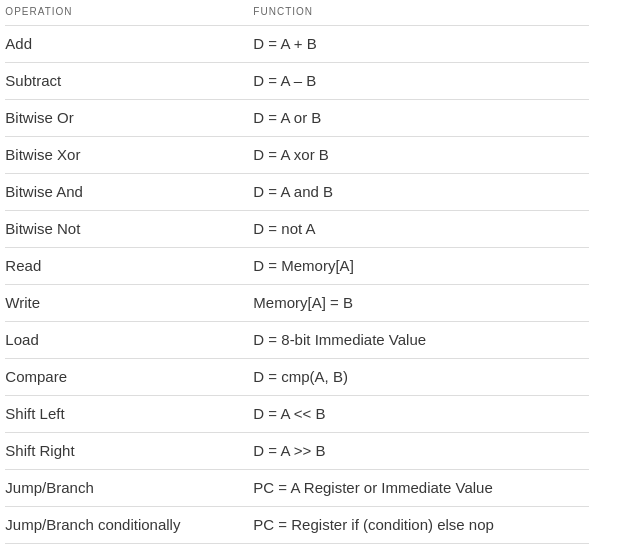
\includegraphics[width=16cm]{Instructions}
\centering
\caption{The Instructions supported by the TPU ISA}
\centering
\label{fig:instr}

\end{figure}


Migen was chosen as the HDL of choice because of its simplicity and Python-like syntax. The ISA supports 14 different instructions. They are the basic and the most found instructions in similar RISC ISAs. The instructions are of three categories 

\begin{enumerate}
\item Arithmetic Instructions : These instructions are basically for basic numeric operations. This include Addition(ADD) and Subtraction(SUB). All other arithmetic instructions such as Division and Multiplication can and would be implemented as a function of some basic instructions
\item Logical Instructions : These instructions are basically for basic Logical operations. They are carried out both on numerical data and logical data. 
\item Conditional and Branching Instructions
\item Memory accessing Instructions:These instructions are very important in the storage and retrieval of data in the memory of a system. They include SAVE, LOAD and WRITE instructions.
\end{enumerate}

There is a need to define the structure of instructions for the ISA. It is a common thing to put the OPCODE first before the ARGUEMENTS of the particular command. An intruction can have a number of arguments or inputs depending on it structure. There are quite a number of ways by which instructions are structured in this regard. This is shown in the Figure \ref{fig:instr}. Some instruction take, as arguements, the regidters number. This means that the operation is performed on the content of the registers and stored in a particular output register. Some other instruction takes the constant inside the instruction and directly perform operation on them. All these depend on the kind of operation to be carried out on the data. 
An instruction is basically a 16-bit nuumber and it contains both the operation and the operands(Register number or constant). The OPCODE is 4-bit wide and is enough for our 14 operations with space left for two more in the future. The OPCODE starts from the 15th bit and ends on the 12th bit. This is consistent across all instructions . The other forms of instruction bit assignment are shown in Figure \ref{fig:inst_bit_srt}. 

\begin{figure}[p]

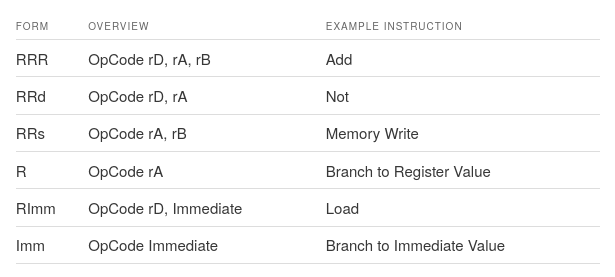
\includegraphics[width=16cm]{opcode_Structure}
\centering
\caption{Instructions Structure.}
\centering
\label{fig:inst_str}
\end{figure}


\begin{figure}[p]

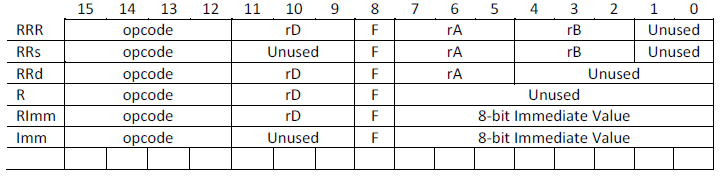
\includegraphics[width=15cm]{forms_bits_organization}
\centering
\caption{Instructions bit Assignments.}
\centering
\label{fig:inst_bit_srt}
\end{figure}

A very important thing to note at this point is the fact that the load value is unable to load into a register a 16-bit value at once. This is because the instruction itself is 16 bit and still has to contain other things like the OPCODE and other parameters just as important as the data. This is remedied by allowing the processor to load into the upper and lower part of a register independently. Thsi is controlled by the bit number eight. This parameter is found in all instructions but used only by very few ones.

It is also important to know that our registers are demoted by three bits of the instruction. This allows for referencing only eight registers. This is a core and intrinsic part of the ISA and cannot be changed wwithout changing the ISA itself.
The processor does not possess a special register for special numbers and special functions such as the Stack pointer in the Beta machine. This greatly simplifies the complexity of the system at the expense of its performance.  

\subsection{Designing the Register File}
The Register File is a part of the processor that contains the registers. There are eight 16-bit individual registers that make up the Register File. The Register File is the storage medium for the processor. It is where data is stored during operation. They are usually made of the fastest kind of memory element to reduce access time during operation. 

The Register Files takes in one 16-bit data inputs and two 16-bit data outputs. These outputs allow data from two different register to be available at the output buses for the ALU. The choice of register is made by the output bus select inputs. These inputs are three bits and are just enough to adderess the eight registers of the register files. The destination of the data on the input bus is also controlled by a write enable bit and a three bit select input. Therefore, data can be written to the Register files when it is needed. Finally, there is a clock input and an enable bit to activate the whole Register file as a whole.

During the implementation of this module, I wrote the program in such a way that the output from the Register File is held until the select pin changes the choice of register. In other words, if the Register File is enabled , it will always output the content of two registers based on their respective select input. I wrote a testbench to simulate every possible scenarios and I was able to make the Register File perform as follows.

\begin{figure}[p]

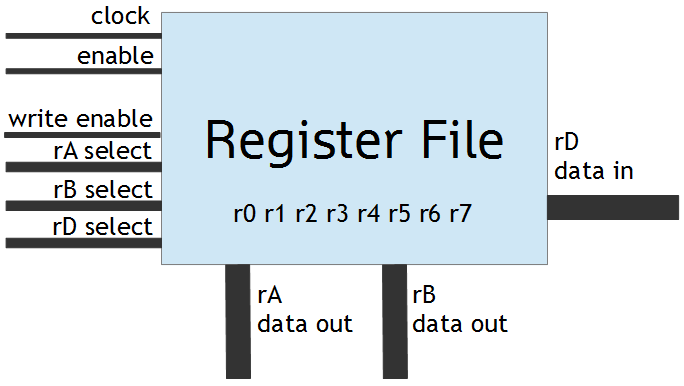
\includegraphics[width=12cm]{reg_file}
\centering
\caption{Diagramatic representation of an Register File}
\centering
\label{fig:decoder}
\end{figure}







\subsection{Designing the Instruction Decoder}
The decoder is a very important section of a microprocessor. it is responsible for extracting necessary data and commands from an instruction. In other words, it is responsible for pulling bits out from the instruction stream and sending them on to the other units we connect to: The Register file, ALU, and Control unit(s).

The Instruction decoder require the fillowing inputs.
\begin{itemize}
\item Clock input
\item An enable input
\item Instruction input
\end{itemize} 

The outputs include the following 
\begin{itemize}
\item the Alu OPCODE.
\item Selection lines for the Register file (rD, rA and rB).
\item Write enable to enable writing into the Register file.
\item The Immediate(Constant) value from the instruction.
\end{itemize}

The ALU OPCODE also contains the flag. The flag signifies different things for different commands. The instructions that require the flag bit make use of it in the code and others that don't simply discard and ignore its existence. For the case of memory based commands like LOAD and WRITE, it is for putting the immediate value in the upper or lower eight bit part of the selected register rD. For that of JUMP, it is for signaling if the processor should jump to the immediate value or to the value stored in the given register. Figure  \ref{fig:opcode_bit_flag} shows the list of the commands, their OPCODES, and the status of the write enable and flag. Figure \ref{fig:decode} shows a diagrametric representation of an Instruction decoder.



%\begin{figure}[p]
%
%
%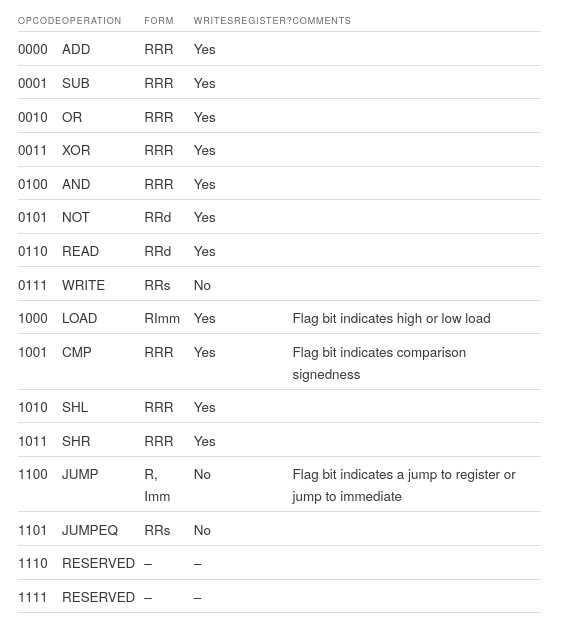
\includegraphics[width=13cm]{opcode_with_flag}
%\centering
%\caption{OPCODES and Instruction Structure.}
%\centering
%\label{fig:opcode_bit_flag}
%
%\end{figure}
%
%\begin{figure}[p]
%
%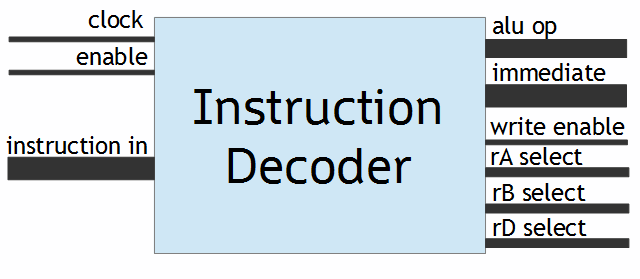
\includegraphics[width=12cm]{decoder}
%\centering
%\caption{Diagramatic representation of an Instruction Decoder}
%\centering
%\label{fig:decode}
%\end{figure}

\begin{figure}[p]
\subfloat[]{
\label{fig:opcode_bit_flag}
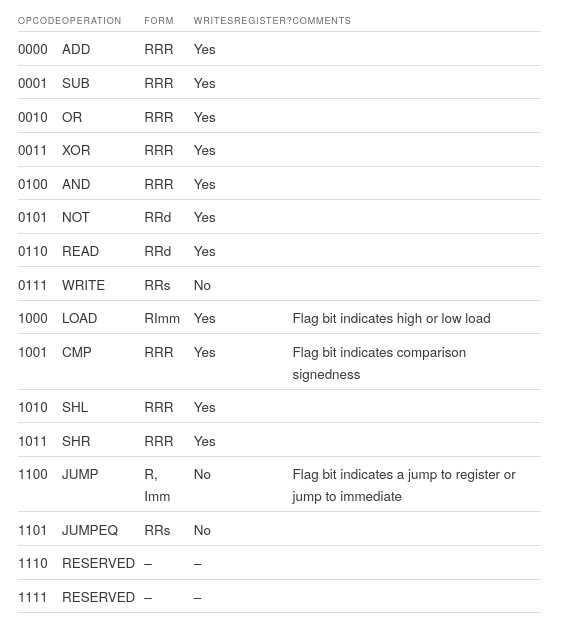
\includegraphics[width=13cm]{opcode_with_flag}
}
\\
\subfloat[]{
\label{fig:decode}
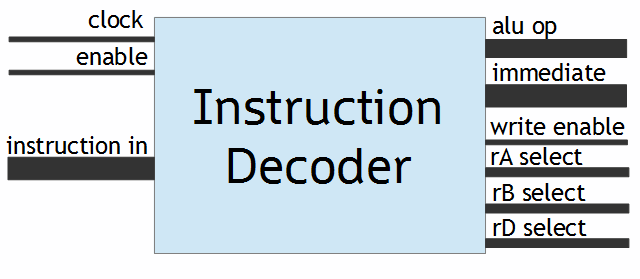
\includegraphics[width=12cm]{decoder}
}
\caption{Diagramatic representation of an Instruction Decoder}
\label{fig:globdecode}
\end{figure}


\subsection{Designing the Arithmetic and Logical Unit}

In TPU, we are only doing single cycle operations. Whilst a whole instruction will take multiple cycles to complete, the ALU itself will output a result in a single clock cycle. The other cycles are due to decoding, fetching and any writebacks of results which are required. The ALU takes in two 16-bit data input, an ALU opcode and produces the output of the operation after a number of clock cycles. 
Other inputs include clock, enable bit, write-enable bit, 16-bit program counter and eight bit immediate value. The program counter and the immediate value inputs are for storing important data required for loading data into the register file. in the case of the program counter, the important data is the next address to go to. This is an important reason for outputing a shouldBranch output bit. This helps to signify when a jump is required during the execution of a particular instruction.

Our ALU process which runs on a rising clock edge, when enable bit is active, will immediately enter a case statement dependent on the alu operation forwarded from the decoder and inputed though the ALUop input. 
Each if block within the case statement will write to elements of an internal register sresult, which is 18 bits wide, to accommodate carry or overflow status. There is also an internal signal for the shouldBranch output.The shouldBranch output is not computed but inferred from the opcode. This is because of the fact that we already know the number of instructions that requires branching. 
The ALU code was written to be as optimized as possible as it - just as others - can cause a serious bottleneck in the operation of the microprocessor.
\begin{figure}[p]
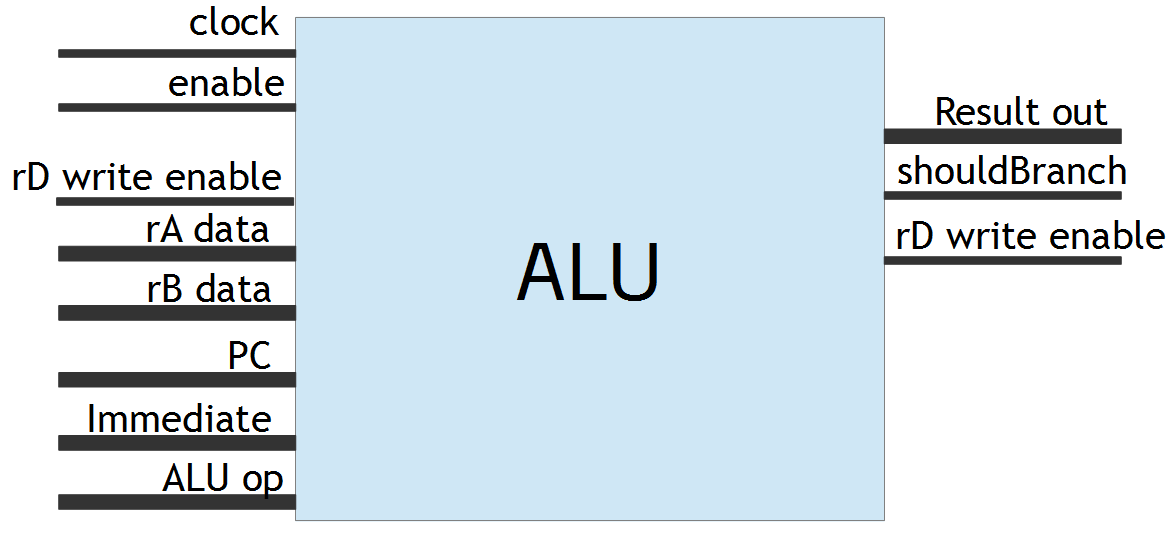
\includegraphics[width=12cm]{alu}
\centering
\caption{Diagramatic representation of the Arithmetic and Logical Unit.}
\centering
\label{fig:alu}
\end{figure}



\subsection{Designing the Control Unit}
During the implementation of the other modules, you will notice the presence of enable bits in all of the modules. This gives us the ability to switch our modules inputs on at will. Each module has a register at its output and it will preserve the output until the enable bit is asserted and the computation is carried out.  
The control unit basically controls the enable bit of every module of the micro processor. it helps in the crude pipelining of data in the processor. 
The control unit is technically a state machine, but for now it’s simple enough we can just classify it as a counter. It is a simple six bit counter. The code was written to shift a bit right through its output and activate the neccessary module. It activates the RAM first since it is where the instruction is fetched and sent to the decoder.


\subsection{Designing the Program Counter}
The Program Counter (PC) is a very important part of a microprocessor. It contains the address (location) of the instruction being executed at the current time.  It helps to simplify the process of jumping and branching to any instruction by allowing this to be done by changing its value.
In the TPU, our PC unit will obviously hold the current PC address, and on command increment it. It has an input for setting the next PC value, and also the ability to stop – stay at the same location – which we need due to our pipeline being several cycles long.

Our PC is basically required to perform one of the following things at a particular time.
\begin{enumerate}
\item Increment PC
\item Set PC to new value
\item Do nothing (halt)
\item Set PC to our reset vector, which is 0x0000.
\end{enumerate}

This means that two bit is enough to tell the PC what to do. This input is the PCin input. The normal state of the PC is when PCin is equal to 0. At this point, the PC simply increments its current value by one as it is the normal feature of programs to execute from top to bottom.

\begin{figure}[p]
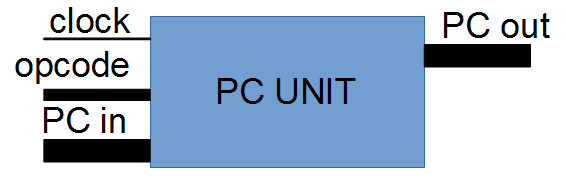
\includegraphics[width=12cm]{pcunit}
\centering
\caption{Diagramatic representation of the Program counter.}
\centering
\label{fig:pcunit}
\end{figure}

\subsection{Simulation and Testing of Different Modules}
During the process of implementing the ISA in migen, modularity was paramount. This led to the independent development of individual modules albiet the fact that they were designed to work together. The pipeline was established and data is meant to progress or move from the program counter to the RAM to the decoder to the register file to the ALU and back to the register file. This flow is controlled by the control unit. 
The individual modules were tested independently and then chained together for a joint test. The testing takes the form of subjecting each module to certain scenarios and checking and confirming that they react and respond in the appropriate ways. The test cases are written in form of testbenchs. The testbenches are written in python and thus inherits the flexibility of python. This is only hindered by the limitation of FHDL itself.

The first module to be tested was the register file. The module was subjected to the following test:
\begin{enumerate}
\item A constant clock input was fed into the module
\item The enable pin was asserted and numbers were stored in different momory location sequentially
\item The numbers were read out of the memory location and compared to the initial stored ones
\item The enable pin deasserted and random numbers were fed into the input in different memory location.
\item The numbers were read out of the memory location and compared to the initial stored ones.
\item Data was stored and retrieved form the register file at the same time in one clock cycle.

\end{enumerate}
At the end of the testing, all scenarios were handled well and the module performed all operation in one clock cycle as intended. The register file passed all the test.
\begin{figure}[p]
    \centering
    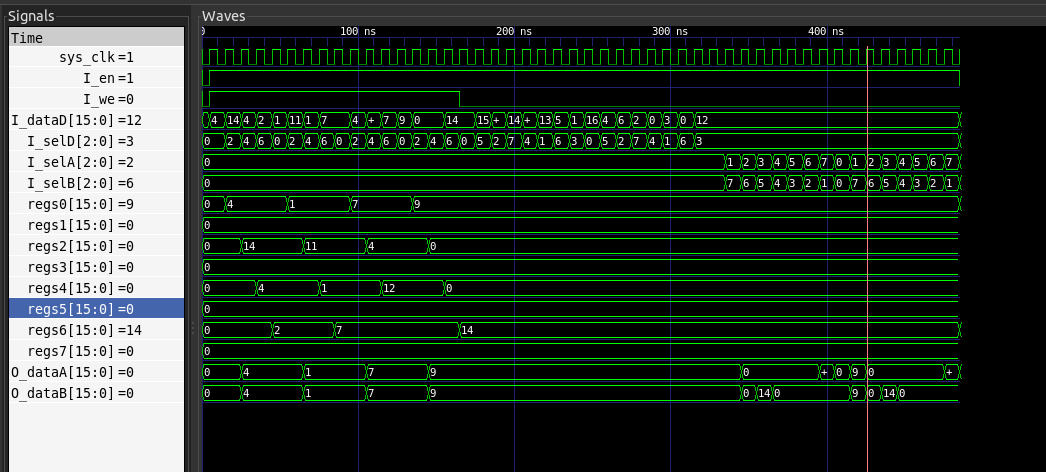
\includegraphics[scale = 0.7]{Reg_file_simulation}
	\caption{Simulation Diagram for an Register FIle.}
    \label{fig:reg_sim}
\end{figure}

The decoder was tested next. Since it is basically meant to extract the embedded data from the instruction and pass them to the neccessary quarters. The module was subjected to the following test:
\begin{enumerate}
\item A constant clock input was fed into the module
\item The enable pin was asserted and i6-bit numbers were passed into the input of the decoder.
\item The individual outputs are manually inspected to confirm that the output  
\item The enable pin deasserted and the same operation tried.
\item I generated a VCD file and displayed the result of the test. This is shown in Figure \ref{fig:Decode_sim}.
\end{enumerate}
The decoder operation was not up to par during the first test. This warranted the need to rewrite the code from scratch after which it passed the test. The instruction decoder performs its operation in one clock cycle.

The Arithmetic and Logical Unit was tested next. The job of the ALU is to take in opcode and perform the action intended on the given operands and output the result. Sometimes, the ALU is simply a transparent gateway through which data pass through to be stored in the register file. 

The module was subjected to the following test:
\begin{enumerate}
\item A constant clock input was fed into the module
\item The enable pin was asserted and numbers and certain opcodes were passed into the ALU inputs.
\item The outputs were read out of the ALU and compared to the required response or result
\item The enable pin deasserted and random numbers were fed into the input.
\item The outputs were read out of the memory location and compared to the initial stored ones.
\end{enumerate}

This operation was iterated for specific instruction opcodes such as ADD, SUB, OR, AND, LOAD, SHL and SHR. Each operation succesfully executed in a clock cycle, maintaining the consistency we have built up with other modules.

The operation of the program counter and the control unit are quite simple and do not really require much testing. The were fed  with clock inputs and their outputs  monitored. At the end of the tests, they gave the expected response in exactly one clock cycle. This would have meant that we have a throughput of a clock cycle.

The individual modules were connected as shown in Figure \ref{fig:TPU_CORE}.

\begin{figure}[p]
    \centering
    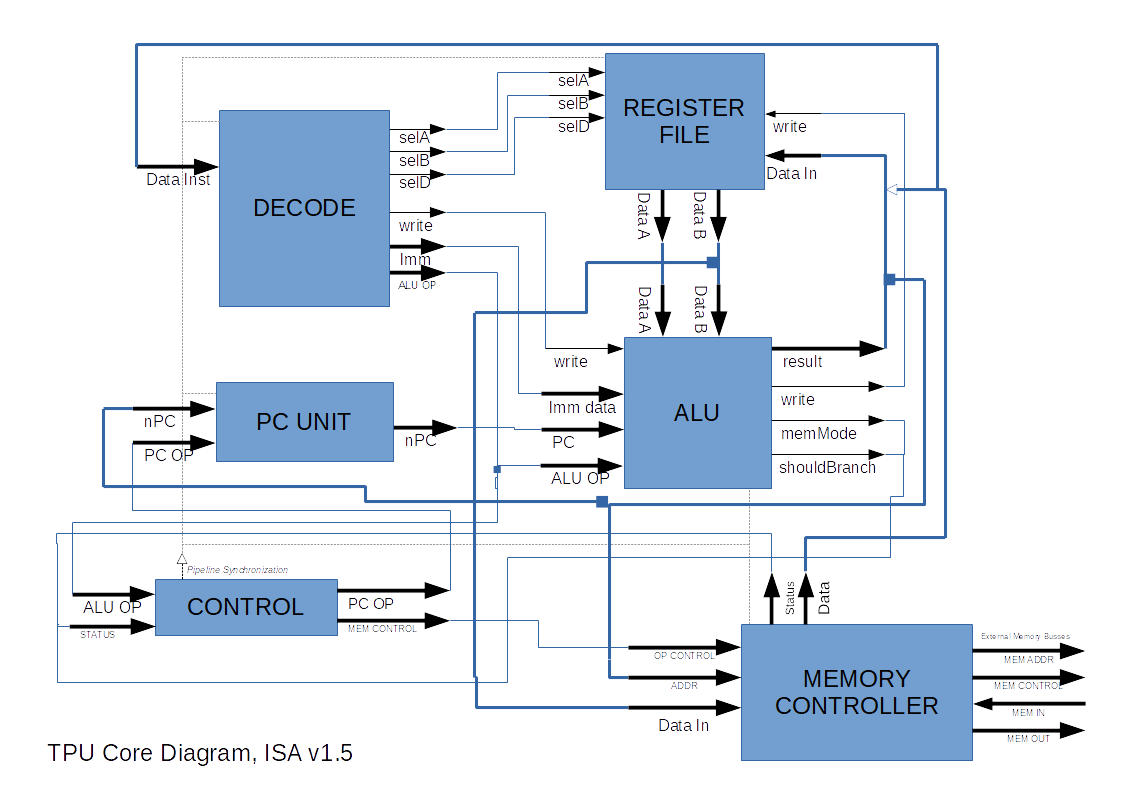
\includegraphics[scale = 0.6]{TPU_CORE}
	\caption{Diagram for an overall connection.}
    \label{fig:TPU_CORE}
\end{figure}
 
Since the testbench is to ba as automated as possible, there became a need for a kind of RAM for storage of instructions. I implemented a scratch pad RAM simply for storage of instructions during initialization of the whole CPU instance.The RAM is 16-bit in width but can take as much as 1024 inputs. This allows for continous operation of the CPU simplifies the test bench to just a series of clock ticks. 

Several instructions were saved in the crude RAM of the processor and allow to run until the end. 
The first set of instructions are as follows:\\
\verb|0x0902| \\
\verb|0x0670|	\\
\verb|0x0902| means \verb|LOAD| \verb|0x02| into register \verb|0x04|.\\
\verb|0x0670| means \verb|ADD| the content of Register \verb|0x03| into the content of register \verb|0x04| and store it in register \verb|0x04|.

\begin{sidewaysfigure}[p]
    \centering
    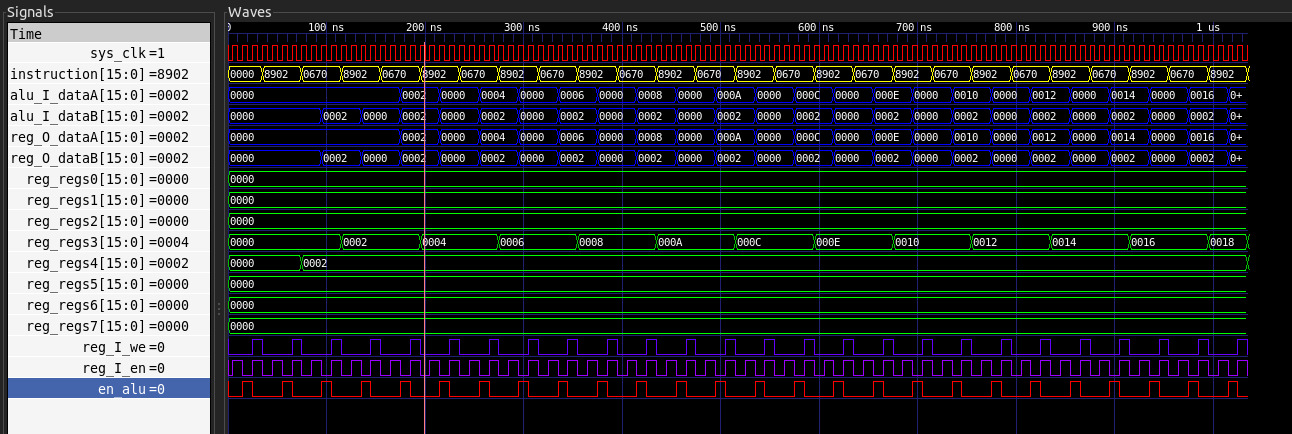
\includegraphics[width=24cm, height=12cm]{CPU_Sim_Control_Unit}
	\caption{Simulation Diagram for MicroProcessor.}
    \label{fig:sim_cpu}
\end{sidewaysfigure}

The result of the testbench as generated by the CPU is as shown in Figure \ref{fig:sim_cpu}.
A very surprising thing that I noticed while going through the simulation diagram is the fact that it takes 6 clock cycles from feeding the pipeline an instruction and getting its output. This came as a shock as I thought that the processor will be outputing data per clock cycle. After looking through the whole architecture, I found out that the states are controlled by the six bit control unit. This means that if there is need to add a new stage to the pipeline, the module to change is the control unit.

Another round of instructions were loaded in the crude RAM. This time, the instructions were as follows:\\
\verb|0x8902| \\
\verb|0x0670|	\\
\verb|0x2A0C|	\\
\verb|0x2A0C| means \verb|ADD| the content of Register \verb|0x02| into the content of register \verb|0x05| and store it in register \verb|0x03| while the other instruction mean the same as the previous test

\begin{sidewaysfigure}[p]
    \centering
    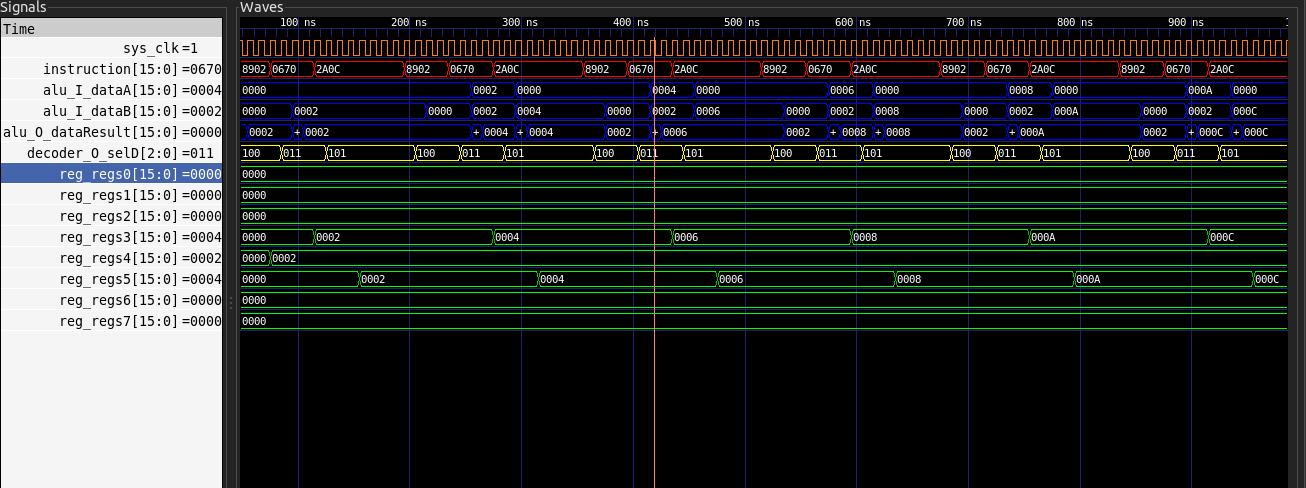
\includegraphics[width=24cm, height=12cm]{CPU_Sim}
	\caption{Simulation Diagram for MicroProcessor instructions Test2.}
    \label{fig:sim_cpu_2}
\end{sidewaysfigure}

The result of the testbench as generated by the CPU is as shown in Figure \ref{fig:sim_cpu_2}. After this test, I noticed that there were some times when the ALU writes to the Register file without the assertion of the Instruction. This lead to a couple of times when the neccessary writebacks dont occur in time and vital info is lost. After a long time of tracking and debugging the code implementation of the TPU, I solved the problem by always keeping the enable bit of the ALU high and adding a latent clock cycle to the pipeline. This means that the TPU will heavily rely on the efficiency of its other modules to make sure the right data is written at the right time. 

A much elaborate test was carried out on the processor with the following instructions:\\
\verb|0x80FE| \\
\verb|0x83ED|	\\
\verb|0x2404|	\\
\verb|0x8701| \\
\verb|0x8902|	\\
\verb|0x0670|	\\
\verb|0x2A0C|	\\
\verb|0xC105| \\
\verb|0x80FE|	\\

\begin{sidewaysfigure}[p]
    \centering
    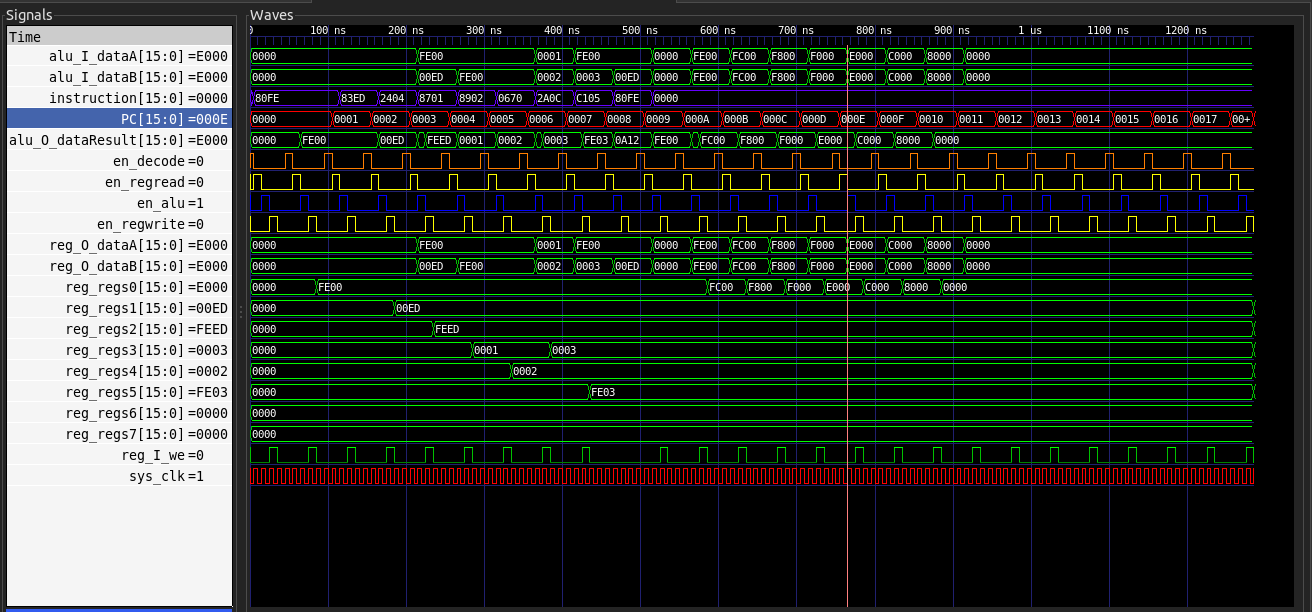
\includegraphics[width=24cm, height=14cm]{PC_implemented_with_enough_latency}
	\caption{Simulation Diagram for MicroProcessor instructions full Test.}
    \label{fig:sim_cpu_3}
\end{sidewaysfigure}

The Figure \ref{fig:sim_cpu_3} shows the instruction loaded inside the RAM and the PC incrementing as required. The activation bits for each stage of the pipeline can also be seen. Although there was a minor glitch in the ALU output at some point, the system rectified this before the activation bit for writeback came around. 

\subsection{Testing on an FPGA}
After testing the modules with testbenches, I flashed the code unto a DE10-Lite Field Programmable Gate Array(FPGA). I wrote a program to count from one to a  thousand, display it on a seven-segment display and light up a LED if the number is prime. This is a considerably tough test for the processor and it is a worthy test of efficiency and validity of most of its commands. The microprocessor, albeit being slow, was able to do this. I also implemented on the FPGA a VGA module and UART module through which the processor communicates with the outside world.




\section[DCU]{Building of a Data Concentration Unit}
GRIT Engineering Limited makes smart utility meters. The current flagship of the company is the G1. This is a smart meter that takes realtime data from the house's electrical network and transmits it to the internet. It is quite efficient but has a few problems. 

One of these problems stem from the fact that it makes use of the popular SIMCOMM's SIM800 module to transmit data to the internet. The availability of network in any particular environment drastically affects the operations of the meter and eventually leads gaps in the data collected from the house. It also defeats the realtime purpose of the smart meter its self. Various network providers have blindspots in their coverage of the entire nation. Altough quite rare, it is possible to have no network coverage in a particular location for hours. The module is also quite expensive as every meter must possess one for it to function as expected. 

Also, the G1 has eight channel for current monitoring and no direct voltage monitoring feature. This leads to the need to fix the voltage for the computations carried out by the device. This fixation of the voltage causes an accumulative error in the data collected as it is quite normal for the line voltage to vary from time to time. The eight channel was also noticed to be quite an overkill as most bulidings do not require more than four to five channels to effectively monitor their useage.

Moreover, the G1 makes use of the popular RaspberryPi Single Board Computer(SBC) for its "heavylifting". The processes that the meter performs are literarily not hard enough to require such complex system as a raspberrypi or any SBC to be frank. Microcontrollers from vendors like STelectronics, Microchip and Espressif have a great reputation for handling these tasks easily and without breaking a sweat while also costing way less than the Raspberrypi. They can even be programmed with Python which is the primary language used in the development of the G1. There is simply no reason to use the raspberrypi anymore.

The need to solve these problems and reduce production cost led to the company's decision to make a new revision of the G1 called the G0. The G0 has the following features.
\begin{enumerate}
\item STM32F407VE Microcontroller based design with low power consumption.
\item Three current sensor port and one voltage sensor port
\item Local Radio transciever for transmitting of data to a data pooling device.
\end{enumerate}
These solved all of the problems enumerated above and also reduced the total cost of making one unit of the device. The device had being designed and made before I resumed work as an intern in the company. The only unfinished job was the communication with a data pooling device which is meant to send the data to the internet.

As a member of the hardware team, I, along with another member of the team, was saddled with the responsibility of designing this important piece of device. It was called a Data Concentrator Unit (DCU). The DCU is basically a custom RF gateway device. It has one RF channel and is to serve all G0 boards in its vicinity. It then will relay the data collected to the internet where it can be viewed and used.

\subsection{Hardware Design}
The requirements given to be satisfied by the DCU is that
\begin{enumerate}
\item It must be power efficient
\item Serve devices within a radius of 700m
\item Internet connected
\item collect data periodically.
\end{enumerate}
  
Due to the following requirements, We decided to use the following components
\begin{enumerate}
\item \textbf{STM32l4 Microcontroller}: The STM32L4 chip is a STElectronic microcontroller that is know for its ability to perform excellently while use=ing very low power. It contains peripherals like Serial peripheral interface (SPI), UART, I2C and a substantial amount of general purpose input/output pins. All these coupled with the fact that it is quite cheap and the company having a substantial amount in stock made the chip the go to for this project. The microcontroller is programmed in C.
\item \textbf{SX1735} The need for radio communication between the DCU and the G0 meters led to the need to use this paricular RF chip. The meter possesses one of this chips and it was only natural for the DCU to have one too. The SX1785 is a radio Frequency Tranciever that communicates via the LoRa modulation technique. This allows for long range of communication with substantial reduction in the power required while also staying unaffected by most barriers.  The LoRa transciever is very cheap and requires an omni-directional antenna to perform effectively. It communicates with the host microcontroller via SPI with speeds up to 4Mhz and supports interrupts on reception of data packets. This means we can easily attend to recieved packets at anytime during operation.

\item \textbf{FerroMagnetic Random Access Memory (FRAM)}: The FRAM is meant to store data recieved from the meters in the case their is no network. Storing the data in the internal flash memory of the microcontroller will only degrade it and make it quite unprdictable in its aged form. The MB16H is a cheap non-volatile memory chip. It has up to Four million write cycles compare with the ten thousand write cycles of Flash. It uses very low power as it does not need to refresh itself once the data is stored. The chip used in this case was MBR16871. Although it was more expensive than flash memory of the same size, it has faster access time and will last longer in operation. 

\item \textbf{18650 Li-ion Battery}: These batteries are very important to the operation of the device. It serves as a power backup in case there is loss of electricity during operation. The 18650 battery is a very common battery found in a lot of products and devices. Its volumetric power ratio is higher than most portable batteries can offer while still being the cheapest of them all. Charging a 18650 Li-ion battery has become very simple and can be done without monitoring due to the emergence of overcharging and short-circuitry protection chips.  They are quite cheap too. 

\item \textbf{SIM800 GSM Module}: The need for this device to pipeline or route data collected from various meters to the internet where they are used and displayed to the end user. SIM800 was a natural choice as the company's webserver has been optimized for recieving requests from them. This is also due to the fact that the 2G network is has quite a wide coverage and is far from being scrapped in a country like Nigeria. It is also quite cheap and has a lot of resources available online and quite easy to get it into operation. 
\end{enumerate}

All the components listed above influenced the decision made during the design of the device. The micro-controller is responsible for directing the operation. It collects data from the LoRa Chip and sends it to the internet via the SIM800 chip. It accesses the FRAM via I2C and stores data unto it in the case of inability to send the data to the internet probably due to network unavailability. The schematic diagram is as shown in Figure \textbf{XXXXXXX}. 

The schematic was implemented in Eagle and sent to china for fabrication. The PCB designed has two layers and uses the conventional FR4 material. All this reduces the cost per unit of manufacturing the device

\subsection{Software Architecture Design}
The hardware being as simple as possible requires intense work with the software architecture to ensure efficient operation. The basic operations that will be carried out by the device are
\begin{itemize}
\item Collect data from meters around it
\item Send the data to the internet
\end{itemize} 
The default state of the meters and the DCU is listening with the LoRa trancievers. This allows for them to use the interrupt capability of the tranciever to collect the data packet, respond and continue what ever the device was initially doing.
A very important feature of the software is the ability to know the number of individual meters it is serving at a particular time and  diferentiate one from the other. During the development of the meter,due to the absence of a SIM800 module, the team could not use the SIM800 IMEI and phone number to identify the meters as used in the previous meters. This led to the generation of an identity number through which one can differentiate one meter from another. These numbers are what we use to coordinate the operations and actions of the DCU.

Foremost, when a DCU is setup in a new environment, it tries to get the identity number of client meters it is serving. It does this by sending a broadcast message containing a certain code to show that all meters in its proximity should respond with their identity number. After making this broadcast, it listens to the response of the meters from which it gets the uniqe identity number of the meters and reply to each of them. The response is needed to assure the meters that their presence has been acknowleged. The DCU will repeat this for two times after which it will send the list of devices to the server. This is to notify the server that timely data for those meeters will henceforth come from this particular DCU.It also saves it on the FRAM for future use.

 
After a succesful setup, the DCU gets data from the meters periodically. This is a variable feature with its default being 30 minutes. The method of collecting data from the is a quite interesting and efficient one. The list of meters necessary to be polled periodically has been previously stored in the non-volatile FRAM. To get the current data from the meters, it broadcasts a message which contains a predefined code for data collection and the identity number of the device. The device being addressed after recieving the message responds with the required data. Every other device do not reply to the message as they have not been addressed.  The DCU goes through this cycle until it exhausts the list on its FRAM. It packages the data and sends it to the server. The advantage of this kind of system is its flexibility. It allows a lot of devices to be addressed and essentially making use if the communication channel like an addressible communication bus. This allows for scalability and increased flexibility.

When a message or data packet is recieved from a meter, a CRC check is performed on it to ensure its integrity.The data is usually is a JSON form.\\
 \verb|{"sn":123456,"t":1538352060,"c":3149,"v":21884,"pf":98,"kw":686881,|\\
 \verb|"kva":714413,"kwh":127,"e-kwh":2922}|\\
If the data is found wanting in any form, the DCU sends a resend code to the meter and it resends the data. The microcontroller used in the DCU is capable of performing CRC checks on data in hardware without breaking a sweat. This helps to speed up the operation. In the case of a new meter winstalled in an environment, it will periodically send out a code to ask to be added to the serve list. The DCU  responds to this by an acknolegement that it has been added after which the meter goes to it normal operation and the DCU updates its saved list. The flow chat of the DCU's program is shown in Figure \textbf{XXXX}

All the features included in the software of the DCU warranted an update to the meters firmware. This was because some features that are of utmost importance to the data collection by the DCU. Unfortunately, the company folded up due to financial issues before the project could be completed.

\subsection{Conclusion}
At the end of the design and prototyping period, the following were achieved.
\begin{enumerate}
\item A multi-client data concentrator unit was developed
\item The DCU is able to route data from its client to the internet
\item The DCU can automatically add new devices to its list of clients
\item The DCU performs error checking on the data packet and can store data in the case of poor network.
\end{enumerate}

The project was a successful one and the basis that I was thought in school was of utmost help.
 
\section{Design of a Gas Monitoring Device} 
A very important and popular part of most kitchen is the gas cooker. It is an efficient burner- cylinder combo that helps cook safely without smoke. It is quite effiicient in operation and the cooking gas is relatively cheap. One problem that comes with using such setup is the fact that it is virtually impossible to know -precisely- the current level of gas in the gas cylinder. The popular way of guessing the amount of gas in the clinder is by weighing with ones arm. This is not efficient but will prepare the person for the eventual exhausting of the gas. One time or the other, we have been left stranded by gas finishing unexpectedly. This is a very bad thing.

The existing solutions to this problem involves the use of scales, digital and analogue. These solutions are not robust enough as they still require the user to constantly check the reading of the scale. It is possible for the gas in the cylinder to finish without the owner noticing a thing. Therefore, there is need for the user to be notified regularly. One of such time should be whenever the gas falls by certain amount. 

GRIT Systems Engineering was contracted with a project to build a cheap gas monitoring device. I was assigned to oversee the design and implementation of the electronic part of the project. This involved choosing a method of gas level monitoring that is cheap, efficient and consume less power. This involved iterating between existing methods of measuring the gas level in a cylnder and settling for one that is easy and cheap to make.


\subsection{Hardware Design}
The following were the necesarry requirements needed to be fufiled by the gas level monitoring device.
\begin{enumerate}
\item It must be power efficient
\item It must collect data periodically and alert users regularly about the level of LPG in the gas cylinder
\item It must be internet connected 
\item It must be cheap and very easy to make.
\end{enumerate}

After reading through a lot of implementations online, weight measurement was chosen over pressure measurement for the gas level monitoring device. This is because measuring weight is less intrusive and cheaper than measuring pressure. The disadvantage is that 
pressure measurement method of gas level monitoring is more accurate that using weights. This disadvantage is one that has no significant on the product as we have quite an acceptable level of tolerance to work with. 

Due to the following requirements, We decided to use the following components
\begin{enumerate}
\item \textbf{ATMega328P} : This is a very common and cheap microcontroller. It is easily programmed in C/C++ with the ArduinoIDE.
This helps reduce the stress needed to develop the device if we were to choose another microcontroller as the Microcontroller has enjoyed a lot of support from the Open Science and Hardware (OSH) community. To cap it all, it is very cheap and has a wide range of peripherals communication hardware like Serial Peripheral Interface (SPI) and I2C.

\item \textbf{Load Cells:} A load cell is a type of transducer, specifically a force transducer. It converts a force such as tension, compression, pressure, or torque into an electrical signal that can be measured and standardized. Strain gauge load cells are the most popular ones you see in a lot of projects. This is because of their cheapness and ease of use. This kind of load cell converts force into resistance and can be measured very easily. This made them the best option for this project. They are usually made in a wheatstone bridge configuration allowing the user to apply an excitation voltage to the circuit and read the small voltage difference across the bridge due to changes in the resistance resulting fro tension on the attached metal strip.

\item \textbf{HX711 :} HX711 is a precision 24-bit analog-to-digital converter (ADC) designed for weigh scales and industrial   control   applications to interface directly with a bridge sensor. Its gain is programmable and is able to read from its two available channels and send the data digitally via a serial data output. This makes it useable by almost any microcontroller with a GPIO. It also has the ability to power down completely when it is not in use. The serial data interface is used for data retrieval, input selection, gain selection and power down controls. It is also quite cheap.

\item \textbf{SIM800 GSM Module}: The need for this device to send data to the internet where it is displated to the end  user. SIM800 was a natural choice as the company's webserver has been optimized for recieving requests from them. This is also due to the fact that the 2G network is has quite a wide coverage and is far from being scrapped in a country like Nigeria. It is also quite cheap and has a lot of resources available online and quite easy to get it into operation. 

\item \textbf{18650 Li-ion Battery}: These batteries are very important to the operation of the device. It serves as the primary power source  during operation. The 18650 battery is a very common battery found in a lot of products and devices. Its volumetric power ratio is higher than most portable batteries can offer while still being the cheapest of them all. Charging a 18650 Li-ion battery has become very simple and can be done without monitoring due to the emergence of overcharging and short-circuitry protection chips.  They are quite cheap too. 

\item \textbf{DS3231 Real-Time Clock} The DS3231 is a low-cost, extremely accurate I2C real-time clock (RTC) with an integrated  temperature-compensated crystal oscillator and crystal. The device incorporates a battery input, and  maintains  accurate timekeeping when main  power to the device is interrupted. The RTC maintains seconds, minutes, hours, day, date, month, and year  information. More importantly, it has two programmable alarms that are linked to a GPIO. This module is necessary because of the need to add time stamps to the data we collect and also wake up the entire system at intervals.
\end{enumerate}
The above list contains the most prominent and important components used in the devices components. The Atmega328p chip, being the brain of the device, directs the operation of the device as a whole. It is connected to the HX711 module via a two wire serial interface bus from which it caliberates and read the current weight of the gas cylinder. The HX711 handles the necessary amplification and analog to digital conversion that is required by the load cell. The microcontroller also communicates with the SIM800 via UART with AT commands. It is through this that it communicates with the internet and send data periodically to the company's server. The microcontroller is connected to the DS3231 RTC by $I^2C$. It is from this chip that it gets the current time and add the timestamp to any data that is to be sent to the data. The whole device is powered by a single 18650 Li-ion battery. The battery, according to given specification, is meant to be changed regularly by authorised technicians hence the absence of a charging circuit for the battery. The 3.3V linear regulator serves the microcontroller, HX711, RTC while the SIM800 module is powered directly from the li-ion battery but controlled by a MOSFET with which we can switch the SIM800 on or off at will. A button is added for caliberation purpose.

The most intriging part of the schematic is the automatic switching of the device. The DS3231 chip as previously mentioned as 2 programmable alarms. When the alarms go off they pull the open drain pin of the RTC chip low. I designed a system by which we can use this feature to great advantage. Since the pin is open drain, it is manually pulled up to 3.3V with a resistor. The same pin is connected to the gate of a P-channel MOSFET which serves as a switch for the whole system. The P-channel is usually, by default, swiched off due to the state of the alarm pin connected to its gate. This means that by default, the whole system is dead. At the preset time, the alarm goes of and the alarm pin is force down to ground. The P-channel MOSFET comes on and allows current through it. This allows the microcontroller and other perpherals to switch on and take the necessary readings. When there is need to switch off the the device, the alarm bit is cleared and the alarm button goes back to its initial state of being HIGH.

It is important to know that the RTC is always on and runs on its coin cell power source during the switch off stage. This allows to extend battery usage time by a long time. There is no better way to save power than to switch off our devices and allow a certifed low power time keeper wake it up at intervals. 

\subsection{Software Architecture Design}
The whole cycle begins with the alarm going off and the whole system getting powered. After initiallization of the several modules and peripherals, the microcontroller takes the current reading of the gas cylinder from the HX711 chip. It then compares the value gotten with a previously collected and stored weight. if the difference between the values is greater than 200 grammes, it powers on the SIM800 module and then sends the data to the company's web server. It also saves the data on its internal EEPROM for use during the next startup. If the difference is not that pronounced, it will simply do nothing. The next thing the device does after the data comparison is to clear the alarm bit after which the whole system is shutdown. This process takes around 15 seconds and is carried out eight times in a day. It helps to reduce the power consumed by the device by constantly collecting data and providing it in real-time to the web server. It helps extend the battery life while ensuring that timely data is still being collected.

The method of comparing weights is relative rather than absolute. This helps to remove variables such as weights of the cylinder from the problem. Using absolute will require us to know the weight of the gas cylinder and we will not need to compare it with previous data. 

\subsection{Conclusion}
At the end of the design and prototyping period, the following were achieved.
\begin{enumerate}
\item A gas monitoring device was developed
\item The device is able to send data periodically to the internet
\item The device can run for a whole year on a single Li-ion cell
\end{enumerate}

The prototype was a successful one. The method of switching the whole system with a RTC was so efficient that I made it into an open source board available online for everyone. The basis of electronics that I was taught in school was of utmost importance and helped scale many hurdles during the development of this prototype.




